\section{Scaling laws 扩展：把预算问题说清楚}

\subsection{compute-optimal}

当 FLOPs 是硬预算时，最关键的问题就变成：是做更大的模型，还是训练更多 token？课程要教你的不是一个死公式，而是如何把它变成可测量、可拟合、可预测的问题。

\begin{figure}[H]
\centering
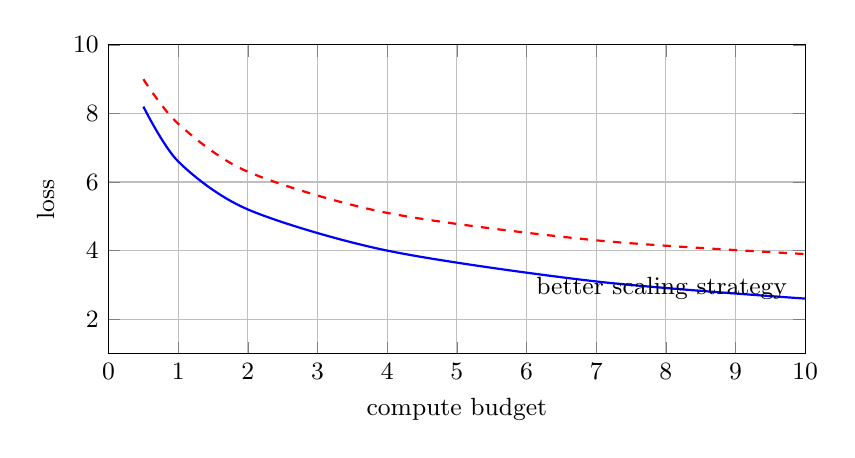
\begin{tikzpicture}[font=\small]
\begin{axis}[
width=0.86\textwidth,
height=5.5cm,
xlabel={compute budget},
ylabel={loss},
grid=both,
xmin=0, xmax=10,
ymin=1, ymax=10
]
\addplot[smooth, thick, blue] coordinates {(0.5,8.2) (1,6.6) (2,5.2) (4,4.0) (7,3.1) (10,2.6)};
\addplot[smooth, thick, red, dashed] coordinates {(0.5,9.0) (1,7.7) (2,6.3) (4,5.1) (7,4.3) (10,3.9)};
\node at (axis cs:6.0,2.9) [anchor=west] {better scaling strategy};
\end{axis}
\end{tikzpicture}
\caption{scaling law 的直觉：同样 compute 下，策略不同，loss 曲线会整体错开}
\end{figure}

\begin{table}[H]
\centering
\begin{tabular}{p{3.0cm}p{4.3cm}p{5.8cm}}
\toprule
\textbf{问题} & \textbf{答案形式} & \textbf{意义} \\
\midrule
更大模型还是更多 token? & tradeoff & 预算分配 \\
如何做小实验? & fit a scaling law & 小规模指导大规模 \\
什么最怕浪费? & expensive compute & 每一块 FLOP 都有机会成本 \\
\bottomrule
\end{tabular}
\caption{scaling laws 要回答的三个预算问题}
\end{table}

\begin{knowledgebox}{scaling laws 的价值}
\begin{itemize}
    \item 让你不靠拍脑袋分配 compute。
    \item 让你知道实验应该做多大。
    \item 让你把“感觉”变成定量策略。
\end{itemize}
\end{knowledgebox}

\subsection{attention vs MLP}

课程用一个朴素例子说明：在小模型里，attention 和 MLP 的 FLOPs 可能差不多；但放大以后，MLP 占比会迅速上升。把时间花在小规模 attention 的微优化上，未必会对最终大模型最关键。

\begin{figure}[H]
\centering
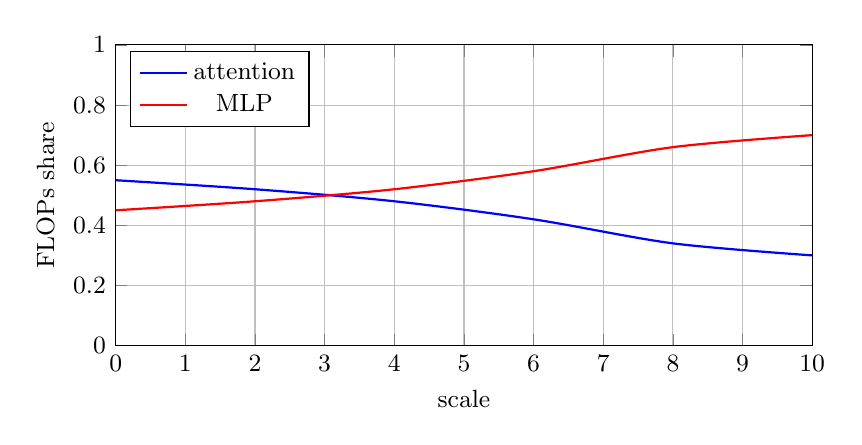
\begin{tikzpicture}[font=\small]
\begin{axis}[
width=0.86\textwidth,
height=5.4cm,
xlabel={scale},
ylabel={FLOPs share},
legend style={at={(0.02,0.98)},anchor=north west},
grid=both,
xmin=0, xmax=10,
ymin=0, ymax=1
]
\addplot[smooth, thick, blue] coordinates {(0,0.55) (2,0.52) (4,0.48) (6,0.42) (8,0.34) (10,0.30)};
\addlegendentry{attention}
\addplot[smooth, thick, red] coordinates {(0,0.45) (2,0.48) (4,0.52) (6,0.58) (8,0.66) (10,0.70)};
\addlegendentry{MLP}
\end{axis}
\end{tikzpicture}
\caption{scale effect 示例：更大规模时，MLP 往往会成为更大的 FLOPs 消耗项}
\end{figure}

